% This is "sig-alternate.tex" V1.9 April 2009
% This file should be compiled with V2.4 of "sig-alternate.cls" April 2009
%
% This example file demonstrates the use of the 'sig-alternate.cls'
% V2.4 LaTeX2e document class file. It is for those submitting
% articles to ACM Conference Proceedings WHO DO NOT WISH TO
% STRICTLY ADHERE TO THE SIGS (PUBS-BOARD-ENDORSED) STYLE.
% The 'sig-alternate.cls' file will produce a similar-looking,
% albeit, 'tighter' paper resulting in, invariably, fewer pages.
%
% ----------------------------------------------------------------------------------------------------------------
% This .tex file (and associated .cls V2.4) produces:
%       1) The Permission Statement
%       2) The Conference (location) Info information
%       3) The Copyright Line with ACM data
%       4) NO page numbers
%
% as against the acm_proc_article-sp.cls file which
% DOES NOT produce 1) thru' 3) above.
%
% Using 'sig-alternate.cls' you have control, however, from within
% the source .tex file, over both the CopyrightYear
% (defaulted to 200X) and the ACM Copyright Data
% (defaulted to X-XXXXX-XX-X/XX/XX).
% e.g.
% \CopyrightYear{2007} will cause 2007 to appear in the copyright line.
% \crdata{0-12345-67-8/90/12} will cause 0-12345-67-8/90/12 to appear in the copyright line.
%
% ---------------------------------------------------------------------------------------------------------------
% This .tex source is an example which *does* use
% the .bib file (from which the .bbl file % is produced).
% REMEMBER HOWEVER: After having produced the .bbl file,
% and prior to final submission, you *NEED* to 'insert'
% your .bbl file into your source .tex file so as to provide
% ONE 'self-contained' source file.
%
% ================= IF YOU HAVE QUESTIONS =======================
% Questions regarding the SIGS styles, SIGS policies and
% procedures, Conferences etc. should be sent to
% Adrienne Griscti (griscti@acm.org)
%
% Technical questions _only_ to
% Gerald Murray (murray@hq.acm.org)
% ===============================================================
%
% For tracking purposes - this is V1.9 - April 2009

\documentclass{sig-alternate}

\begin{document}
%
% --- Author Metadata here ---
\conferenceinfo{ROSS}{'11 Tuscon, Arizona USA}
%\CopyrightYear{2007} % Allows default copyright year (20XX) to be over-ridden - IF NEED BE.
%\crdata{0-12345-67-8/90/01}  % Allows default copyright data (0-89791-88-6/97/05) to be over-ridden - IF NEED BE.
% --- End of Author Metadata ---

\title{XCPU3}
\subtitle{Workload Distribution and Aggregation}
%
% You need the command \numberofauthors to handle the 'placement
% and alignment' of the authors beneath the title.
%
% For aesthetic reasons, we recommend 'three authors at a time'
% i.e. three 'name/affiliation blocks' be placed beneath the title.
%
% NOTE: You are NOT restricted in how many 'rows' of
% "name/affiliations" may appear. We just ask that you restrict
% the number of 'columns' to three.
%
% Because of the available 'opening page real-estate'
% we ask you to refrain from putting more than six authors
% (two rows with three columns) beneath the article title.
% More than six makes the first-page appear very cluttered indeed.
%
% Use the \alignauthor commands to handle the names
% and affiliations for an 'aesthetic maximum' of six authors.
% Add names, affiliations, addresses for
% the seventh etc. author(s) as the argument for the
% \additionalauthors command.
% These 'additional authors' will be output/set for you
% without further effort on your part as the last section in
% the body of your article BEFORE References or any Appendices.

\numberofauthors{3} %  in this sample file, there are a *total*
% of EIGHT authors. SIX appear on the 'first-page' (for formatting
% reasons) and the remaining two appear in the \additionalauthors section.
%
\author{
% You can go ahead and credit any number of authors here,
% e.g. one 'row of three' or two rows (consisting of one row of three
% and a second row of one, two or three).
%
% The command \alignauthor (no curly braces needed) should
% precede each author name, affiliation/snail-mail address and
% e-mail address. Additionally, tag each line of
% affiliation/address with \affaddr, and tag the
% e-mail address with \email.
%
% 1st. author
\alignauthor
Eric Van Hensbergen \\
       \affaddr{IBM Research}\\
       \email{bergevan@us.ibm.com}
% 2nd. author
\alignauthor
Pravin Shinde \\
       \affaddr{ETH Zurich}\\
       \email{pse220@few.vu.nl}
\alignauthor
Noah Evans \\
       \affaddr{Alcatel-Lucent Bell Labs}\\
       \email{noah.evans@plan9.bell-labs.com}
}

\maketitle

\begin{abstract}
TBD: One paragraph summary, this paper can't fit any more than that.
\end{abstract}

\section{Introduction}

The deluge of huge data sets such as those provided by sensor
networks, online transactions, and petascale simulation provide 
exciting opportunities for data analytics.  
The scale of the data makes it increasingly difficult to process 
in a reasonable amount of time on isolated machines.
In the near future petascale and exascale simulation will make 
the involvement of secondary storage and disks impractical, driving
the need for infrastructures which provide in-situ analytics and
visualization capabilities~\cite{ma:in-site}.

Our experiences with existing tools for constructing dataflow workflows
for simulation, transformation, analysis and visualization were frustrating.

* tight coupling of language, runtime, and workflow methodology
* overly complex and difficult to deploy on petascale clusters or 
dynamic resources
* primarily targeted at post-processing

%This has lead to data flow systems emerging
%as the standard tool for solving research problems using these vast
%datasets.  In typical dataflow systems,
%runtimes~\cite{dean2008msd}~\cite{bialecki:hfr}~\cite{isard2007ddd}
%~\cite{streamit} and  define graphs of processes, the edges of the graphs
%representing pipes and their vertices representing computation on a
%system.  Within these runtimes a new class of
%languages~\cite{pike2005idp}~\cite{yu2008dsg}~\cite{olston2008pln} can
%be used by researchers to solve "pleasantly parallel" problems(problems where the individual elements of datasets are considered
%to be independent of any other element) more quickly without worrying
%about explicit concurrency.
%
%These languages provide automated control flow(typically matched
%to the architecture of the underlying runtime) and channels of
%communication between systems.  In existing systems, these workflows
%and the underlying computation are tightly linked, tying solutions
%to a particular runtime, workflow and language.  This creates
%difficulties for analytics researchers who wish to draw upon tools
%written in many different languages or runtimes which may be available
%on several different architectures or operating systems.

We observe that UNIX pipes were designed to get around many of these
incompatibilities, allowing developers to hook together tools written
in different languages and runtimes in ad-hoc fashions.  This allowed
tool developers to focus on doing one thing well, and enabled code
portability and reuse in ways not originally conceived by the tool
authors.  The UNIX shell incorporated a model for tersely composing
these smaller tools in pipelines (e.g. 'sort $|$ uniq -c'), creating
coherent workflow to solve more complicated problems quickly.  Tools
read from standard input and wrote to standard output, allowing
programs to work together in streams \emph{with no explicit knowledge
of this chaining built into the program itself}.

One to one pipelines such as those used by a typical UNIX shell,
can not be trivially mapped to streaming workflows which incorporate
one-to-many, many-to-many, and many-to-one data flows.  Additionally,
typical UNIX pipeline tools write data according to buffer boundaries
instead of record boundaries.  As \cite{pike2005idp} notes dataflow
systems need to be able to cleanly separate input streams into
records and then show that the order of these records is independent.
By separating input and output into discrete unordered records data
can be easily distributed and coalesced.

To address these issues we have implemented a prototype shell, which
we call PUSH, using dataflow principles and incorporating extended
pipeline operators to establish distributed workflows ---potentially
running on clusters of machines--- and correlate results.  
%Our
%implementation is based on extending an existing shell, MASH\cite{mashman},
%from which we inherited a rich interpreted scripting language.  It
%treats variables as lists of strings and has no native handling for
%any other data type.  Integer expression handling and other facilities
%are provided by shell commands.  It has native regular expression
%support and it has a novel ability to do declarative shell programming
%through a make like syntax incorporated in the shell itself.
%
%We currently have a working prototype of the PUSH shell, which we
%can use to target local distributed clusters, dynamic clusters built
%using Amazon's EC2 cloud, and large scale clusters such as a Blue
%Gene running the kittyhawk infrastructure.  We are currently in the
%process of evaluating and optimizing performance for a variety of
%application types.
%
%the RC shell\cite{rcpaper} to easier integration into traditional unix
%systems like Linux. This version is simplified and closer to the
%bourne shell. The explicit goal of the new version of Push is
%integration with the Unified Execution Model(UEM)\cite{van-unified} which will
%allow the transparent distribution of processes and the connection
%of their communication channels between machines transparently.
%This work is taking place as part of the HARE project\cite{van2008holistic} 

This paper is organized as follows. The next section 
covers our core design elements of the PUSH shell and the distributed
infrastructure we use to deploy PUSH workflows on systems ranging from
single nodes to bluegene.  Section 3 will discuss some of the implementation
details and experiences of our initial prototype.  In Section 4 we will 
evalute the overhead of our infrastructure and in section 5 we will discuss
the results and explore opportunities for improvement in both the design
and implementation of our approach.


\section{Desgin}

\begin{figure}[htp]
\centering
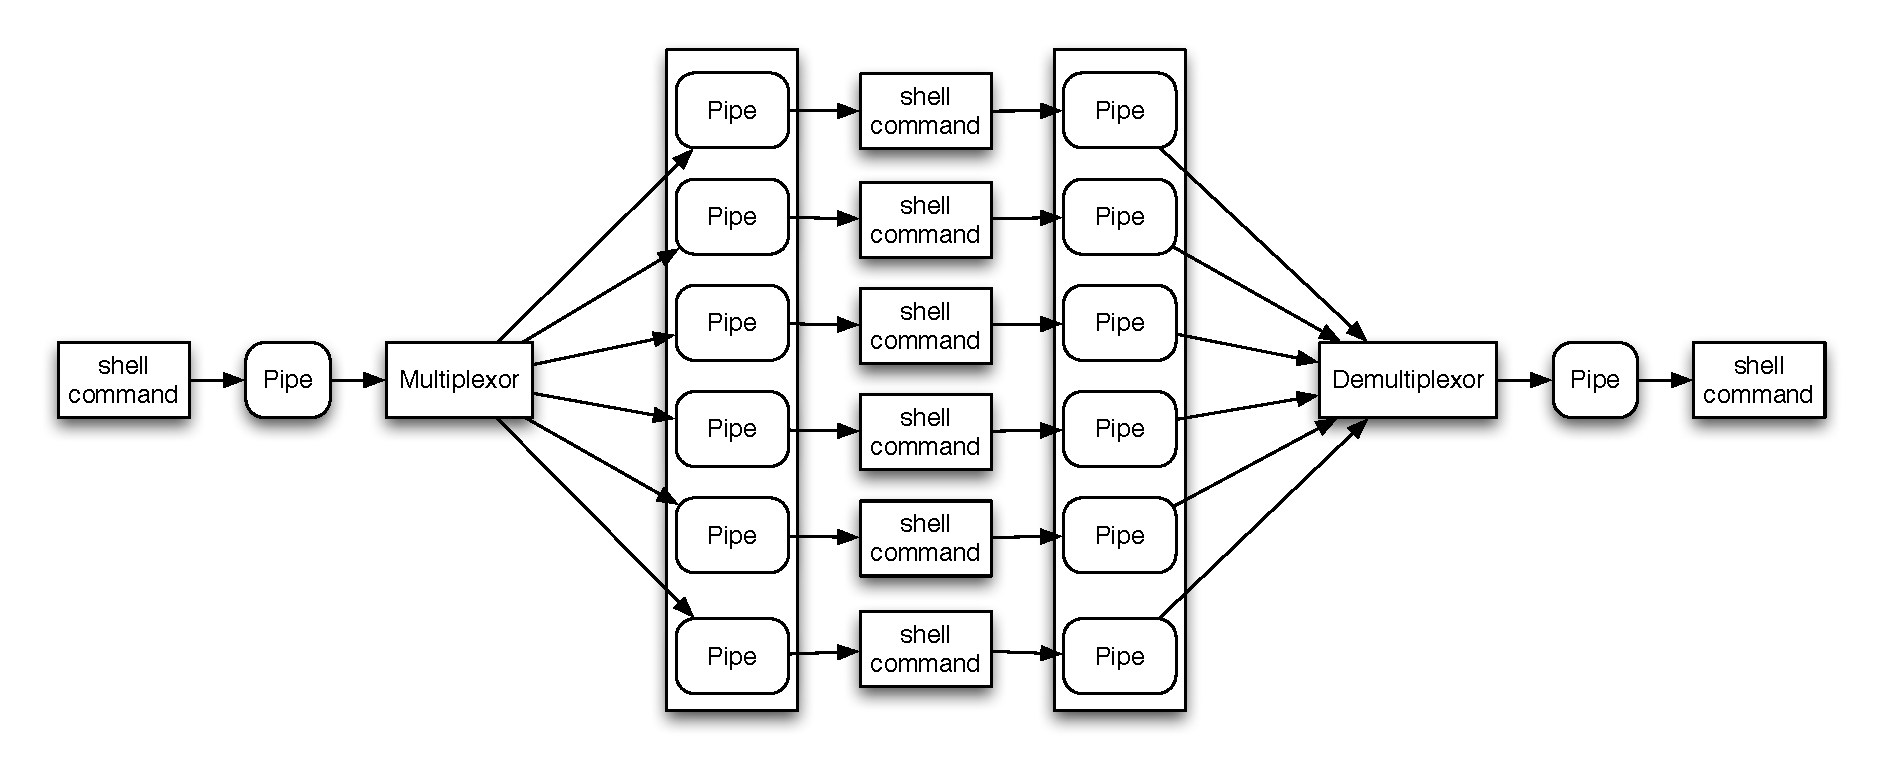
\includegraphics[width=3in]{pipestruct.eps}
\caption{The structure of the PUSH shell}
\label{fig:pipestruct}
\end{figure}

The PUSH shell is a conventional UNIX shell with 
two additional pipeline operators, a multiplexing 
fan-out(\verb!|<![\emph{n}]), and a coalescing fan-in(\verb!>|!).
This combination allows PUSH to distribute I/O to and from multiple
simultaneous threads of control.
A fan-out argument, \emph{n}, specifies the desired degree of parallel
threading.  If no argument is specified, the default of spawning a new
thread per record (up to the limit of available cores) is used.  This can
also be overriden by command line options or environment variables.
The pipeline operators provide implicit grouping semantics allowing natural
nesting and composibility.
While their complimentary nature usually lead to symmetric
mappings (where the number of fan-outs equal the number of fan-ins), there is
nothing within our implementation which enforces it.
Normal redirections as well as application specific sources and sinks
can provide alternate data paths.

PUSH also differs from traditional shells by implementing native support for
record based input handling over pipelines. This facility is similar to the
argument field separators, IFS and OFS, in traditional shells which use a
pattern to determine how to tokenize arguments. PUSH provides two variables,
ORS and IRS, which point to record separator modules. These modules
(called multiplexors in PUSH) split data on record boundaries, emitting
individual records that the system distributes and coalesces.
The choice of which \emph{multipipe}, an ordered set of pipes, to target is
left as a decision to the module.

Different data formats may have different output requirements.Demultiplexing from a multipipe is performed by creating a many to one
communications channel within the shell. The shell creates a reader processes
which connects to each pipe in the multipipe. When the data reaches an
appropriate record boundary a buffer is passed from the reader to the shell
which then writes each record buffer to the output pipeline.

% EVH: the example here may be superfluous as its really just justifying
% map/reduce, not the particulars of the PUSH implementation.
An example from our particular experience, Natural Language Processing, is
to apply an analyzer to a large set of files, a "corpus". User programs go
through each file which contain a list of sentences, one sentence per line.
They then tokenize the sentence into words, finding the part of speech and
morphology of the words that make up the sentence.
There are a large number of discrete sets of data whose order is not 
necessarily important. We need to perform a computationally intensive task 
on each of the sentences, which are small, discrete records and ideal target 
for parallelization.

PUSH was designed to exploit this mapping. For example, to get a histogram of
the distribution of Japanese words from a set of documents using chasen,
a Japanese morphological analyzer, we take a set of files containing sentences
and then distribute them to a cluster of machines on our network. The command
is as follows:
%
% This example is horribly complex, I favor a more simple formulation
% even if its faked a bit
%
%push -c '{
%  ORS=./blm.dis  du -an files |< xargs os \\
%   chasen | awk '{print \$1}' | sort | uniq -c \\
%   >| sort -rn
%}'
\begin{verbatim}
ORS=blm find . -type f |< \\
xargs chasen | sort | uniq -c >| sort -rn
\end{verbatim}

The first variable, ORS, declares our record multiplexor module, 
the intermediary used to ensure that the input and output to 
distributed pipes are correctly aligned to record boundaries. 
In many cases a default which splits based on atomic writes can
be used or one of several built-ins which split based on a field
separator or newline can be used.

emph{find . -type f} gives a list of the files
which are then "fanned out"(\verb!|<!) using a combination
of a multipipes, and a \emph{multiplexor}
which determines which pipes are the targets of each unit of output.
This fanned out data goes to xargs on new threads
which then uses the filenames as arguments to
chasen. The find acts as a command driver, fanning out file names to the
individual worker machines. The workers then use the filenames input to
xargs, which uses the input filenames as arguments to the target command.
Using the output of the analyzer (Japanese words) are then sorted and 
counted using uniq.  Finally these word counts are "fanned in"(\verb!>|!) 
to the originating machine which then sorts them.

While PUSH works perfectly well on a stand-alone machine, the original
intent was to use it to drive workloads and workflows across a cluster of
machines.  In particular, we were interested on deploying on leadership
class high performance computing machines and as such
a key requirement for us was scalability to a large number of nodes.  
In order to accomplish this we designed the system without any central
component which required knowledge of the entire system.
All knowledge is distributed and then aggregated at certain points.
Descisions like scheduling and job management are also made in a
distributed fashion, utilizing the hierarchy of aggregation points
to eliminate the need for all-to-all communication during workload
distribution.

Instead of traditional client/server models we opted for a peer based
model where every node within the system is capable of initiating new
workflows of computation and managing the newly created pipeline.
This allows workflows and component applications to initiate new branches
of computation or analysis at any stage of the pipeline or in reaction to
data produced by a previous portion of the pipeline giving the entire
infrastructure a degree of elasticity that seemed to missing from 
previously available tools.

In order to scale such a system we decided to go with a hierarchical
organization of nodes.  The aggregation points primary responsibility...
TODO: talk about aggregation in a bit more detail

TODO: discuss command based aggregation/treespawn

TODO: discuss I/O based aggregation

TODO: talk about logical and physical hierarchy mappings

TODO: Multi-Participant Pipelining (aka Splice)

\section{Implementation}

\subsection{Brasil}

\subsection{Central Services}

\subsection{Interface}

\subsection{Filters}


\subsection{Examples}
While the PUSH shell handles much of the complexity of interacting with the
Brasil infrastructure, it is useful to see examples of how it interacts
with the underlying infrastructure in order to understand the various mechanisms
better.  These examples are given from the perspective of directly interacting
with the infrastructure file systems from a normal UNIX shell.

The first example presents how the default aggregation behaviour of Brasil can
used to deploy large number of applications.

\begin{verbatim}
$ less ./mpoint/csrv/local/clone
0 
\end{verbatim}
The above command is an example of creating a new session. The contents read
from the \texttt{[clone]} file represent the session-ID.  Now we use session 0
for performing actual execution.
\begin{verbatim}
$ echo "res 4" > ./mpoint/csrv/local/0/ctl
$ echo "exec date" > ./mpoint/csrv/local/0/ctl
$ cat ./mpoint/csrv/local/0/stdio
Fri May 7 13:53:58 CDT 2010
Fri May 7 13:53:58 CDT 2010
Fri May 7 13:53:58 CDT 2010
Fri May 7 13:53:58 CDT 2010
$
\end{verbatim}
The first echo command sends the request for reserving 4 remote resources. The
next echo command submits the request for executing the \texttt{date} command.
And the \texttt{cat} command on \texttt{[stdio]} returns the aggregated output
to the user.  This example shows all the complexities about finding, connecting
and using the remote resources is hidden behind the filesystem interface.
This approach can be used in the \textit{trivially parallelizable applications}
where the same application is deployed on all the nodes.

When constructing more complicated dataflow pipelines, Brasil handles
reserving the resources and setting up the pipe endpoints of the pipeline
components.
Instead of interacting with the aggregation points, dataflow applications (such
as the PUSH shell) can interact directly with the subsessions responsible for 
each pipeline component.

In this example, we will try to create a small pipeline of two commands
\texttt{date | wc}.  But we will create this pipeline across multiple nodes. 

Lets assume that session 0 is created by opening \texttt{[clone]} file as shown
in the previous example.  The following commands will create the desired
pipeline.

\begin{verbatim}
$ echo "res 2" > ./mpoint/csrv/local/0/ctl
$ echo "exec date" > ./mpoint/csrv/local/0/0/ctl
$ echo "exec wc" > ./mpoint/csrv/local/0/1/ctl
$ echo "xsplice 0 1" > ./mpoint/csrv/local/0/ctl
$ cat ./mpoint/csrv/local/0/1/stdio
1 6 29
$
\end{verbatim}

The first command \texttt{[exec date]} is sent to 0'th sub-session and the
second command \texttt{[exec wc]} is sent to the 1st sub-session.  The
\texttt{[xsplice 0 1]} request tells the parent session to redirect the output
of the 0'th session to the input of the 1st session.  The \textbf{xsplice}
command can be seen as a pipe operator of the shell script for redirecting the
output of one command to the input of other command.

The above example is equivalent of executing \texttt{date | wc} on the shell,
but with the difference that both commands are executed on a different remote
machines while sharing the same namespace.


\section{Overhead Evaluation}
\emph{TODO: The big thing to do in this section is rework wording and
hopefully add a splice overhead evaluation. It would also be nice to
change the initial experiment to execution only (no input or output)}.

In order to assess the overhead of our execution deployment and communication
mechanisms as scale, we deployed our infrastructure on a BlueGene/P system
with resources provided by the Department of Energy's INCITE program.
For the purposes of our initial prototype we limited our evaluation to a
BlueGene/P configuration with only 512 nodes (comprising 2048 cores).
We run hosted Inferno on the PowerPC Linux based controller node and on
the Plan 9 based I/O and Compute nodes.
The user interacts with the Brasil instance via shell scripts which 
interact with file system interfaces exported by Inferno and mounted 
under linux with the v9fs file system.

\subsection{Execution}

Our first objective is to meaure the overhead of deployment and execution
of pipeline components as the number of components increases.  Since we 
are only interested in the overhead of deployment we chose to execute the
\texttt{date} command as our example pipeline component.
This is a small application which does not require any external inputs 
and produces small output. 
While this is hardly a characteristic workload, its short execution and
minimal requirements will give us a better sense of the latency overheads
of the infrastructure versus measuring the performance of any particular
applicaiton.
Each deployment involves
session creation, reservation, execution, output aggregation and termination.

\begin{figure}[h]
  \begin{center}
    \leavevmode
      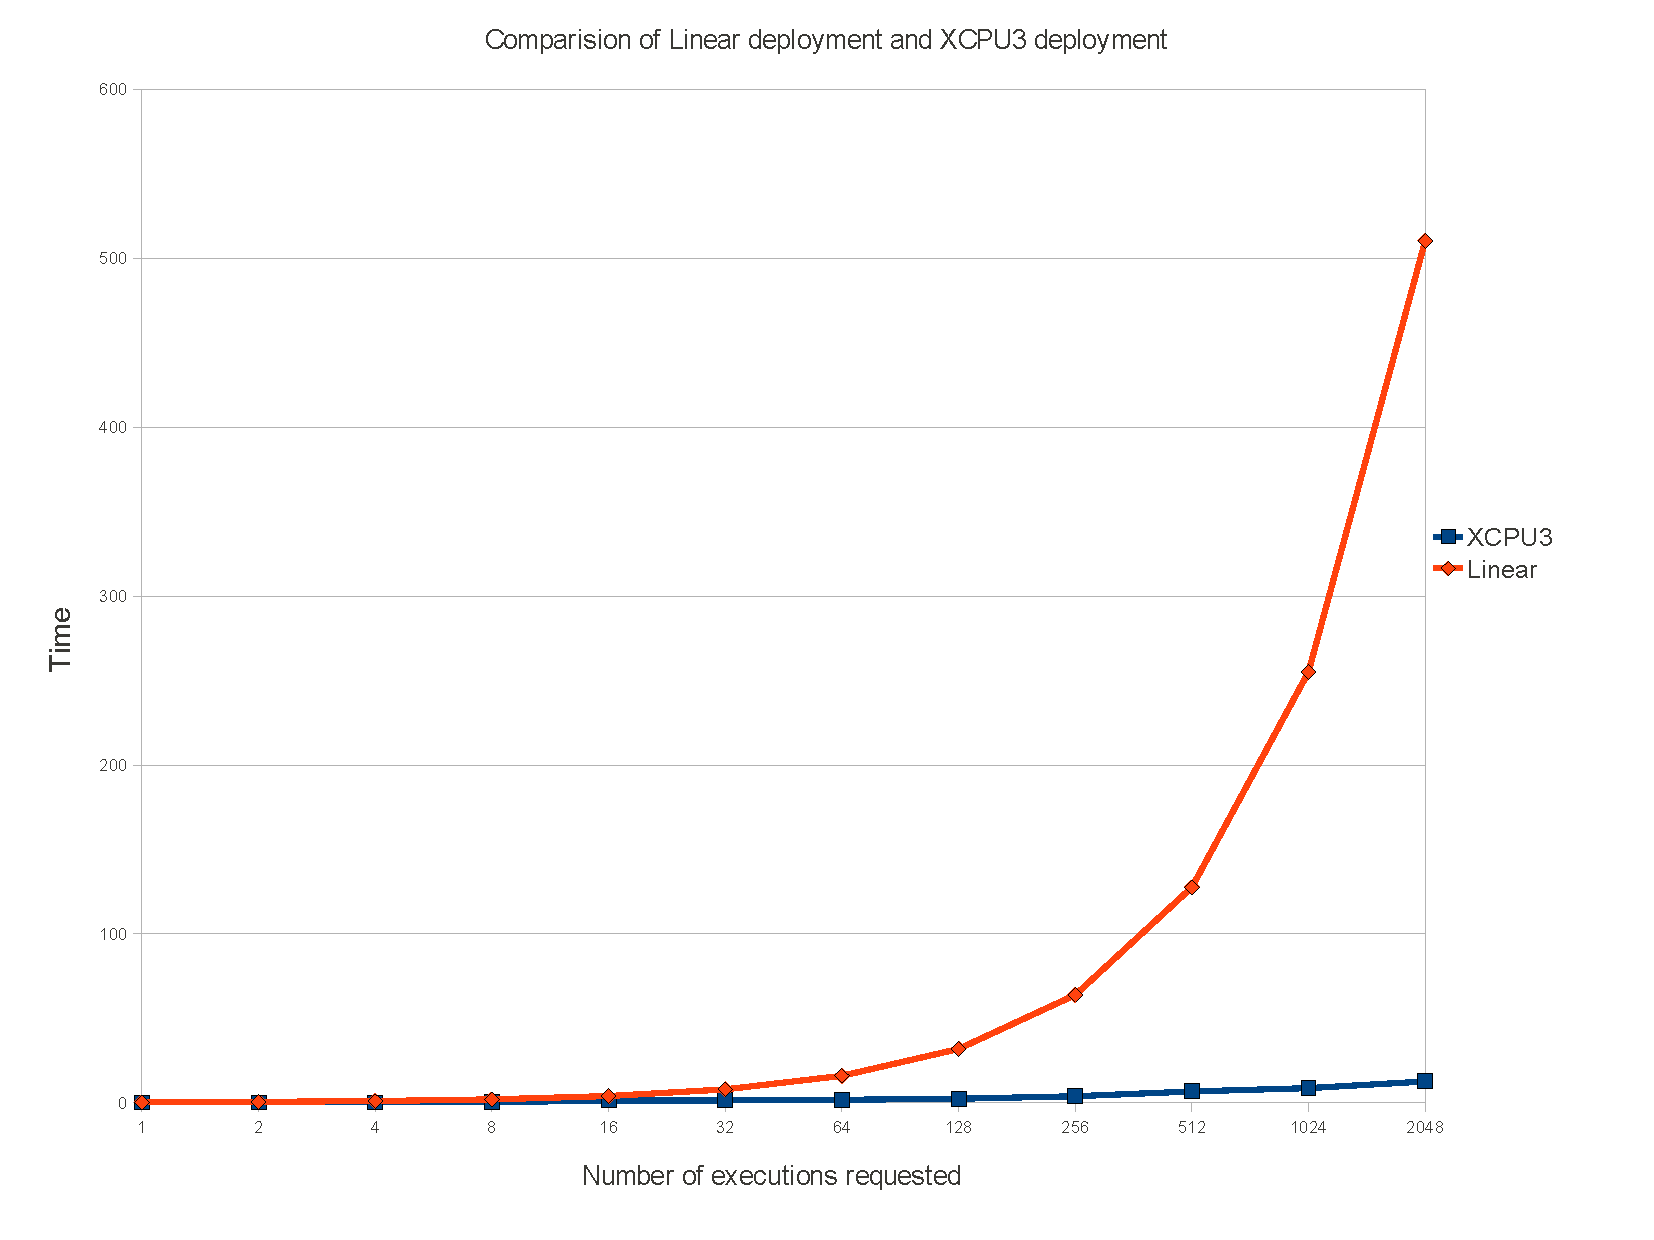
\includegraphics[height=0.2\textheight,width=0.5\textwidth]
		{./img/linear}
    \caption{Comparison if Brasil with sequential deployment}
    \label{fig:sequential}
  \end{center}
\end{figure}

%
% We may end up losing this graph as its kinda bogus
%
Figure \ref{fig:sequential} gives an initial perspective of how Brasil performs
relative to sequential performance.  This graph plots the total time taken by
Brasil and the hypothetical time it may take for performing the same amount of
work on one machine.  This graph shows that the Brasil is successfully able to
exploit the parallelism for deploying the jobs quickly. The Brasil deploys 2048
jobs in 12.66 seconds whereas sequential execution would take upto 510 seconds.
In the graph, the line showing sequential scaling looks exponential, but that is
because number of requested executions increase exponentially.

\subsection{Communication}

This section aims to further analyze the performance of Brasil.  Again we are 
concentrating on similar deployment.  We have recorded the time taken by each
of the following stages in the deployment on the Brasil infrastructure.

\begin{enumerate}
\item Reservation: Create a new session, and request the reservation by writing
\texttt{res n} into the session \texttt{[ctl]} file.  Here \textbf{n} varies
from 1 to 2048 representing the number of executions requested. 

\item Execution: Request the execution by writing \texttt{exec date} into the
session \texttt{[ctl]} file.

\item Aggregation: Collect the output generated by all the executions by reading
the session \texttt{[stdio]} file.

\item Termination: Closing all the files and terminating the session.

\item Housekeeping: Additional time taken before, between and after above steps.
\end{enumerate}
Every deployment starts with the creation of the session followed by the
reservation, execution, aggregation and then ending with termination of the
session.  We have taken the average value over multiple runs for our analysis.

\begin{figure}[h]
  \begin{center}
    \leavevmode
      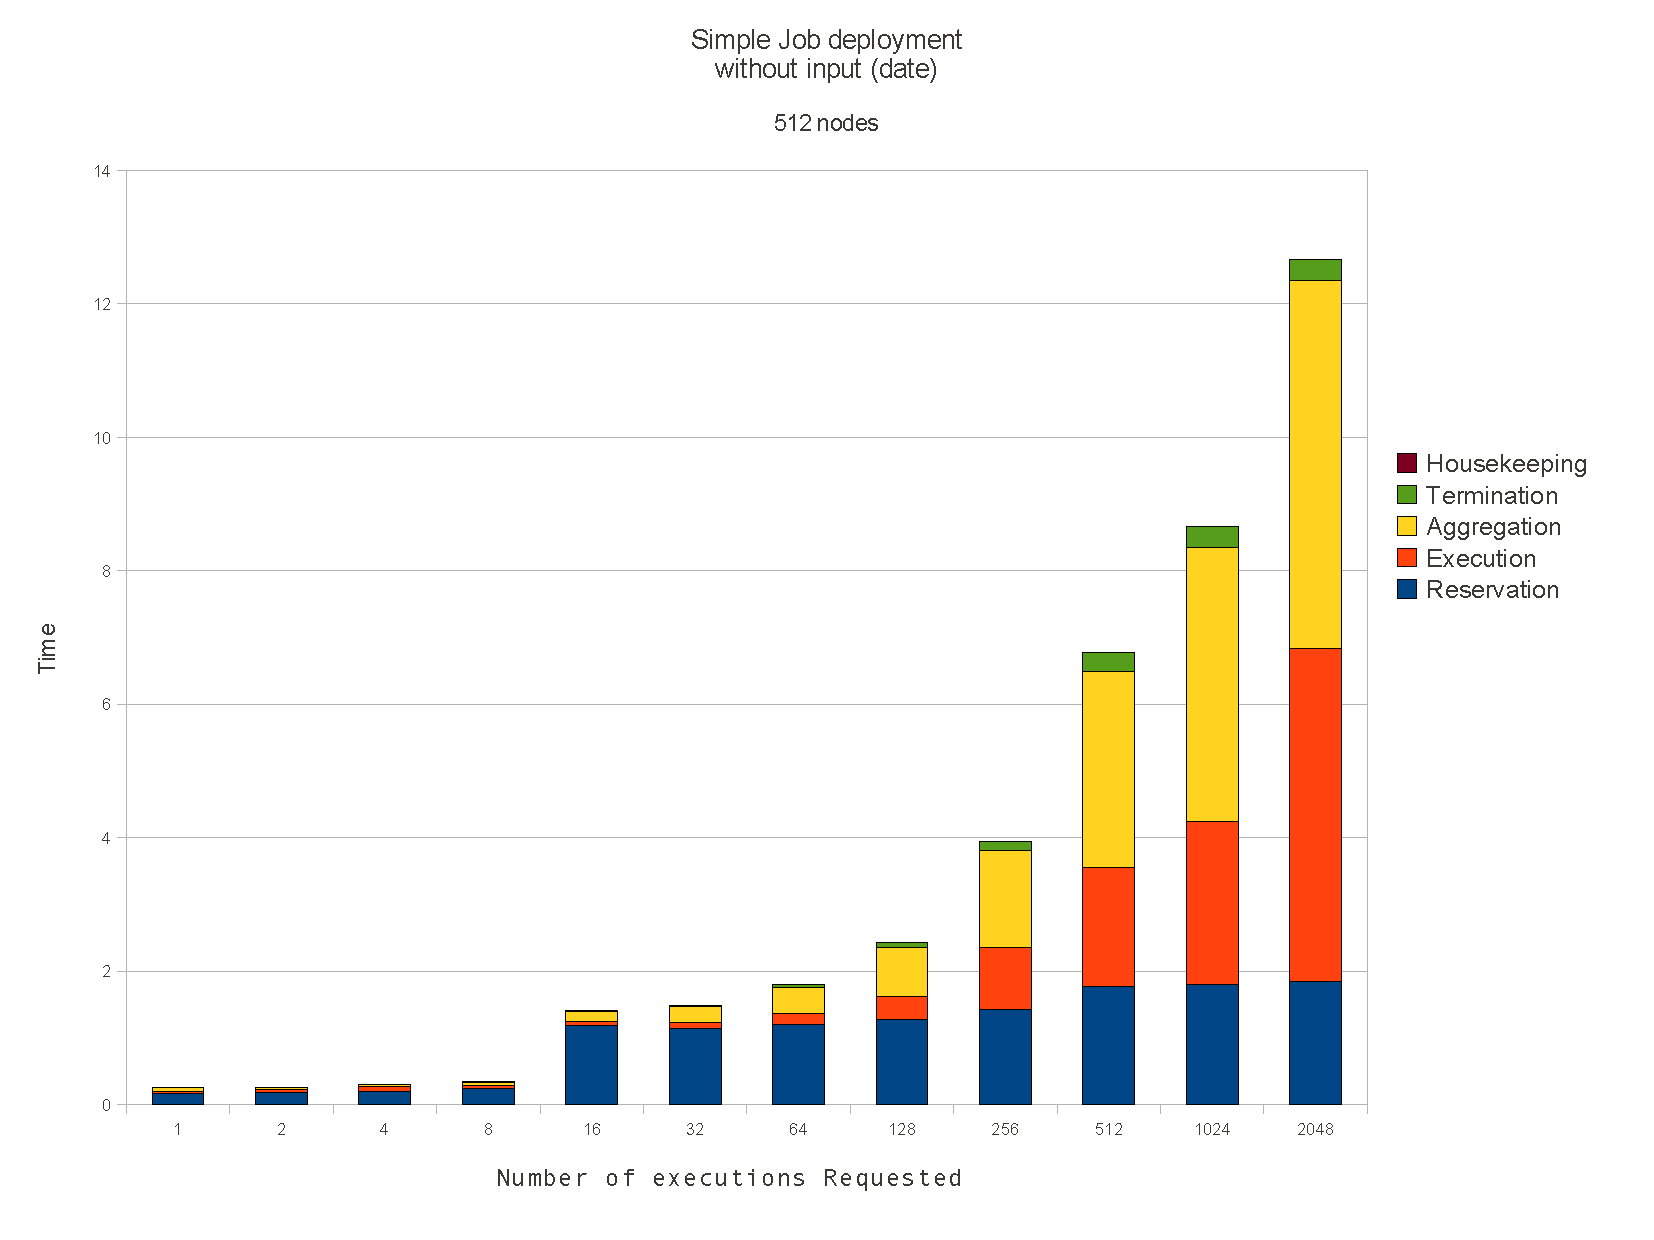
\includegraphics[height=0.2\textheight,width=0.5\textwidth]
		{./img/date_graph}
    \caption{Deployment without input}
    \label{fig:date_graph}
  \end{center}
\end{figure}

Figure \ref{fig:date_graph} presents the results of deployment of the date
command in the form of graph.  This graph presents the breakup time for various
stages of the deployment using the Brasil infrastructure.

From this graph we can observe that the session termination and the housekeeping
overheads are negligible compared to the time taken by reservation, execution
and aggregation.  So, we can ignore these two overheads in our future
evaluations.  For jobs of up to 128 deployments, the reservation time dominates
everything else.  But for larger numbers of deployment execution and
aggregation time increases rapidly while reservation time remains relatively
constant. This shows that reservation time is not directly dependent on
the number of deployments, whereas execution and aggregation time are directly
proportional to the number of deployments.

Now, let us try to analyze why reservation time is independent of the number of
deployments.  The reservation process involves traversing the underlying
topology tree of nodes till the reservation requirements are satisfied.  All the
children on the same level are traversed parallelly at the same time.  This way,
each level is traversed in the constant time, independent of number of nodes in
that level.  Another aspect of the reservation mechanism which helps here is
that the amount of data written and read from the \texttt{[ctl]} file and the
amount of data exchanged between nodes for communicating reservation request is
fixed in size and independent of the number of deployments requested.  With
these two properties, the reservation time becomes directly proportional to the
depth of the tree and not with the number of nodes.

We can observe the above relation in figure \ref{fig:date_graph}. The 
reservation time remains relatively constant for deployment requests from 1 to
8.  Then it sharply increases between 8 to 16 and remains almost constant for
all the requests between 16 to 2048.  This can be attributed to underlying
cluster topology. Figure \ref{fig:hare} shows the presence of the 8 IO nodes
in the first level. This enables satisfying the requests which are smaller
than 8 executions. For larger requests, one more level needs to be traversed
in the topology, introducing delays.  The time taken for reservation remains
almost constant between 16 and 2048 executions as all these reservation
requests essentially traverses the same depth.  We can conclude from these
observations that \textit{the time taken for the reservation is directly
proportional to the depth of the tree}.

Now let us discuss, why the same property is not exhibited by execution time or
aggregation time. We have discussed in the implementation chapter that all
read and write requests are performed in parallel between all the nodes in the
same level.  But the amount of data exchanged for aggregation and execution is
not constant.  This data is directly proportional to the number of nodes
involved.  With the increase in the number of requested deployments, the
amount of data to be exchanged also increases, leading to larger aggregation
time. The execution time is also similarly affected as all compute nodes will
try to fetch the binary of the executable from the initiating node leading to
the copy of the data. These observations lead us to to conclusion that
\textit{the time taken for the execution and aggregation is directly
proportional to the number of deployments requested}.

Our next evaluation involve the deployment of an executable \texttt{wc} which
needs input. This command counts the number of lines, words and characters in
the input file.  This is an interesting case for our infrastructure as this
deployment involves the distribution of inputs to all the sessions.  This
introduces a new stage in the deployment process in addition to the 5 stages we
described in the above section.  This stage will be the \textbf{input} stage and
involves distributing the input data to all the sessions which are responsible
for execution.  By default Brasil will broadcast the input to all the compute
nodes, but we have plans to introduce filters in the PUSH shell which can
partition the input given to the compute  nodes. 

Figure \ref{fig:wc_graph} presents the results of evaluations involving the
distribution of the input.


\begin{figure}[h]
  \begin{center}
    \leavevmode
      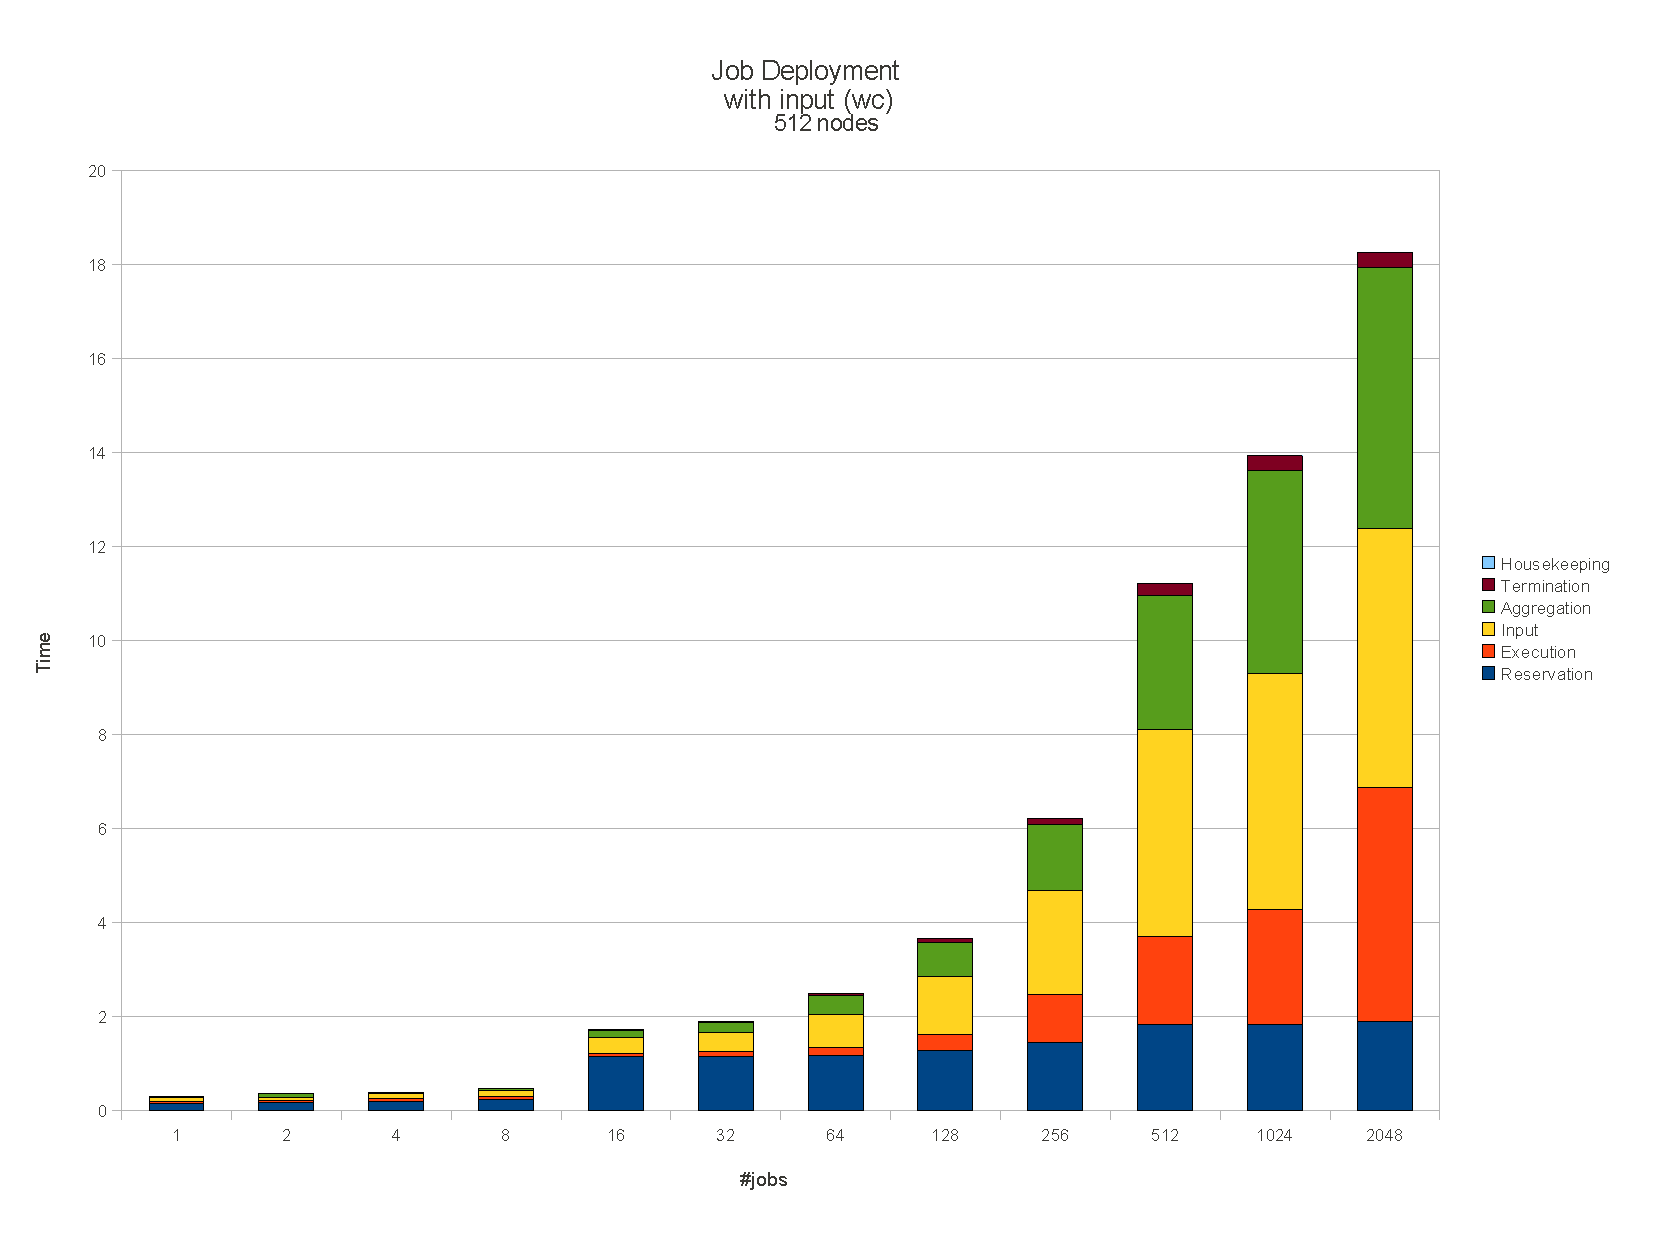
\includegraphics[height=0.2\textheight,width=0.5\textwidth]
		{./img/wc_graph}
    \caption{Deployment with input}
    \label{fig:wc_graph}
  \end{center}
\end{figure}

These results enforce our observations that reservation time is directly
proportional to the the depth of the tree whereas aggregation and execution time
are directly proportional to the number of deployments requested.  In addition
to these observations, we can also observe that the input time exhibits 
behavior similar to the execution and aggregation time.  This observation can be
attributed to the fact that input distribution implementation is similar
to the output aggregation implementation.  And also the amount of data to be
exchanged for input distribution depend on the number of deployments requested
as this data needs to reach all sessions responsible for execution.  This
increases the amount of data to be exchanged with any increase in the number of
the deployments requested.  We can conclude with this observation that
\textit{the input time is directly proportional to the number of deployments
requested}

\subsection{Dataflow}
The evaluations presented in this chapter helps us in understanding how fast
Brasil can deploy small jobs and aggregate the results produced by them.  Now
let us relate how these observations can justify our claims about dataflow
applications. Typical deployments of the dataflow applications are similar to
the above experiments as it involves starting up a large number of small jobs.
But the similarity is over at this point. Dataflow deployment does not always
involve the input distribution and output aggregation stages.  These deployments
work by feeding the output of one computation as input for other computation. 
At the end of the computation, a user needs to read the output of only selected
compute sessions which does not need any aggregation.  What we can conclude from
the above description is that Brasil performs really well in the stages like
reservation which are important for dataflow deployments.  The stages like input
distributions are output aggregation where Brasil is relatively slow are not
needed by dataflow deployments.  This makes Brasil ideal for rapid deployment of
dataflow workloads.

Unfortunately we do not have concrete measurements and evaluations to back our
predictions.  Brasil is one of the piece in the envisioned solution for problem
of efficient and easy deployment of large-scale dataflow applications.   We are
still working on the integration of userspace applications like
PUSH\cite{PODC:Push} with Brasil which will further simplify the dataflow
deployment.

Brasil is an infrastructure which provides the needed flexibility, speed and 
ease of use for dataflow workloads.  This chapter demonstrates the speed that
can be achieved.  It is difficult to measure the properties like \textit{ease of
use} and \textit{flexibility} but the examples presented in the filesystem
interface chapter should give some insights of all the possibilities opened up
by the Brasil.


\section{Discussion}

While our initial experiences with using Brasil to deploy
workloads was positive, we found several areas for improvement
in both the design and implementation of the infrastructure.

One systemic flaw involved the design decision to give the PUSH
shell responsibility for orchestrating record seperation and 
multiplexing.  In enviornments with a lot of communication 
adding additional components to the I/O processing pipeline 
increases overhead due to increased data copying and context
switching.  By moving record seperation into the infrastructure
itself (particularly for common default cases) we can eliminate
a pipeline stage (two copies and two context switches).  By moving
multiplexor functionality into the infrastructure we remove an
additional pipeline stage (two copies and two context switches).
This reduces the overhead of interacting with the infrastructure 
from 6 copies and context switches down to 2.  Taking advantage
of techniques such as Willem de Bruijn's Beltway Buffers~\cite{beltway}
may reduce this even further.

Another unforseen performance problem was caused by the overhead
incurred by the transitive mount methodology of central services.
While elegant, it introduces overhead at each transitive mount point.
As such, deep hierarchies and large scale workloads can involve 
many transitive hops for every communication which introduces latency
and load across the system.  We have identified the need to augment
our hierarchical aggregation (which works well for fan-out and fan-in)
with cut-through models of communication for data-flow operations.
There may also be opportunities to leverage the collective network
capabilities of high performance systems such as BG/P to further
optimize aggregate communication behavior.

While fan-in and fan-out aggregation models do match a large class
of use-cases we quickly found outselves wanting more primitives to
support deeper pipelines and more complex workflows.  In addition
to the two existing extended pipes we identified the need for
deterministic delivery to/from a particular endpoint as well as
many-to-many multipipes.  We also quickly found the need to
incorporate some form of synchronization into the infrastructure
and even came up with ways of doing MPI-style collective operations
using abstract pipeline constructs.

A key failure of our implementation is that it not only lacked
fault tolerance, it lacked good methods of identifying where
in a distributed pipeline failures actually occurred.  Early
debugging was plagued with workflows which would just hang
waiting on input or waiting to give output.  The multi-stage
pipelines present within each PUSH pipeline component further
complicated this.  Part of these problems are inherent in the
way traditional UNIX pipelines work, but we are now experimenting
with "rejoinable" pipelines, task-based workqueue models, and
looking into opportunities for pipeline based work-stealing and
failover in order to alievate workflow stalls.  Additionally,
we are adding new out-of-band logging and error reporting
mechanisms which attach at the same points as the I/O pipelines,
but are used by the infrastructure to communicate failures.

Early on we had a lot of trouble with stalling due to trying to
perform dataflow operations in a synchronous manner.  We later
decoupled these operations into asynchronous threads within
Brasil, but this introduced a number of race conditions which
made traditional pipe semantics difficult to maintain.  We are
left with the opinion that the only way to successfully implement
multipipe semantics is to introduce control sequences to the 
pipelines to assist with identification of when communication
begins and ends.  This detracts from the elegance of pipeline
based solutions, but it also prevents a host of race conditions
and spurious failures.  The good thing is that the complexity 
of dealing with these out of band control messages is hidden 
entirely within the infrastructure, hiding the details from
the end user.

In addition to the design and implementation flaws mentioned
above we realized there were several missed opportunities in
the approach we took with our initial prototype.  
As mentioned in the evaluation section, one of the larger
components of execution time is the loading of the application
binary over the distributed file system.  Given the hierarchical
aggregation of the infrastructure we should be able to provide
more efficient access to binary files and libraries.  A 
straightforward approach is to provide cache capabilities at
aggregation points, but a more aggressive concept is to
incorporate the idea of collective file system pre-fetching
based on session behavior utilizing underlying interconnect
hardware features.  Regardless of implementation, we'd like
to hook distributed file system semantics and capabilities
in more tightly with the infrastructure in the future.

Another set of features we overlooked in our initial 
implementation was adding capabilites which facilitated
more dynamic behavior within sessions or within the
infrastructure itself.  In future implementations we
plan to have a more seamless approach to nodes entering
and leaving the infrastructure, which should enable
cloud deployments and also ease issues with fault tolerance.
In addition to dynamic behavior of the infrastructure, we
also want to better support dynamic behavior within the
workflow.  The existing infrastructure supports spawning
new workflows within the cluster as part of a workflow,
but it would also be nice for workflows to be able to
dynamicly request and release resources from their own
workflow based on workload phase or dependencies
within the data stream.

The experience of implementing the Brasil infrastructure
made it clear to us that the key concept at the core
of PUSH and Brasil was that of the multipipe.  While we
originally only used multipipes as the basis for implementing the
communication aggregation primitives, it became clear to
us that with a few extensions  we could reimplement the 
control plane and monitoring subsystems in terms of 
multipipes as well.  Given the general usefulness of
the multipipe construct we feel it may be a reasonable
candidate for addition to the core operating system 
instead of just being part of a service daemon.  As
such we are currently investigating implementations which
add multipipes as a core system primitive to the Plan 9
and Linux operating systems and reimplementing the Brasil
infrastructure using the new core system primitive.

Our current work as well as our past prototypes are
avaialble as open source via 
http://bitbucket.org/ericvh/hare.


\section{Acknowledgements}
This work was supported in part by the Department of Energy
Office of Science under award number DE-FG02-08ER25851.

\bibliographystyle{plain}
\bibliography{references}

\end{document}
